% Build from the repository root so the bibliography and figures resolve.
\documentclass[conference]{IEEEtran}
\usepackage[T1]{fontenc}
\usepackage{amsmath}
\usepackage{cite}
\usepackage{graphicx}
\usepackage[hidelinks]{hyperref}
\hypersetup{
  pdftitle={Capacity Limits and Second-View Acquisition in Retinal Screening Research},
  pdfsubject={QSART-X author-review draft}
}

\title{Capacity Limits and Second-View Acquisition in Retinal Screening Research}
\author{\IEEEauthorblockN{QSART-X author-review draft}
\IEEEauthorblockA{16 November 2026}}

% These supplementary links resolve to the audited research release commit.
\newcommand{\evidencelink}[2]{%
  \href{https://github.com/Riteshhai/Retina-Opthalmology/blob/a6b4b2b05ff87071f2c0682de78c398e0691a1a3/#1}{#2}}

\begin{document}
\maketitle

\begin{abstract}
We examined specialist-review and recapture capacity under a frozen diabetic
retinopathy policy on 396 photographs from 99 patients in DeepDRiD Set-C, a
held-out split of the same data release. In a separate Set-A analysis, we
fitted a ridge estimator for second-field acquisition on 424 eyes from 212
patients and evaluated it on 84 eyes from 42 different patients. In Set-C,
the deployed ordinal policy overloaded at 30\%, 60\%, and 90\% image review
capacity and recommended review for all 99 patients at full capacity. All 12
policy pairs matching image and patient workloads made identical decisions.
At eight extra fields, the value ranking missed six referable eyes compared
with eight using the first view alone. All 16 equal-acquisition cost
intervals included zero. An acquire-above-estimated-cost rule selected
four fields and retained eight missed referable eyes. These results
quantify the workload cost of full ordinal inclusion and leave comparative
acquisition benefit uncertain.
\end{abstract}

\begin{IEEEkeywords}
diabetic retinopathy, fundus photography, conformal prediction, limited review
capacity, adaptive image acquisition
\end{IEEEkeywords}

\section{Introduction}
Screening evaluations can report both discrimination against released grades
and the workload created by deferral. QSART distinguishes three possible
recommendations: provisional automatic non-referable disposition, image
recapture, and specialist review. Recapture and review draw on separate
resources. QSART-X extends this evaluation with a held-out patient-level replay
and a second-field acquisition analysis. We ask whether constrained allocation
changes decisions at comparable realized workloads and whether first-field
features identify eyes that benefit from a second recorded field. DeepDRiD
provides eye-level diabetic retinopathy (DR) grades, image-level quality
annotations, and fields centered on different parts of the same eye~\cite{R01}.

\section{Materials and Methods}

\subsection{Cohorts and Reference Labels}
The regular-fundus Set-A manifest contains 848 fitting photographs from 212
patients, 168 selection photographs from 42 patients, and 168 calibration
photographs from 42 patients. Included patients contributed two fields per eye
and two eyes per patient. The previously analyzed Set-B confirmation remains
historical internal evidence. The Set-C audit identified a cross-split retinal
fingerprint candidate. The locked protocol excluded all four photographs from
that patient before scoring the eligible 396 photographs from 99 patients.
The reference patient grade is the worse released eye grade. We define grades
2--4 as referable and grades 3--4 as severe for both studies.

The Set-C protocol fixed the model, calibration, gates, and budgets before
scoring. The paired-view value estimator used Set-A fitting patients. Its
evaluation used different patients who had already contributed to selection of
the frozen classifier. The paired-view study used fitting and selection data
only. The calibration partition and the held-out and external cohorts supplied
no fitting or evaluation samples to that analysis.

\subsection{Frozen Predictions and Uncertainty}
Both experiments used frozen first-pass MobileNetV3-Small grading and quality
checkpoints~\cite{R08}. We retained the existing preprocessing and production
temperatures. Temperature scaling divides logits by a positive scalar before
softmax~\cite{R05}. Sums of the corresponding grade probabilities give
referable and severe risk scores. The Set-C conformal analysis fitted a
dedicated temperature on 21 calibration patients and estimated score
thresholds on 21 separate calibration patients. The ordinal and
least-ambiguous classification (LAC) thresholds used the maximum view-level
nonconformity within each calibration patient. At nominal $\alpha=0.10$ we
measured empirical inclusion per photograph and simultaneous inclusion of
all four views per patient.

\subsection{Capacity-Constrained Recommendations}
For a batch of $N$ photographs, the policy applies separate integer caps
$\lfloor B_{\mathrm{review}}N\rfloor$ and
$\lfloor B_{\mathrm{recapture}}N\rfloor$. Review guards use predicted grade,
referable and severe probabilities, predictive entropy for adequate-quality
photographs, and the optional prediction set. In the ordinal and LAC
conditions, a set containing a referable grade or an empty set triggers
review. Poor-quality photographs without a mandatory review trigger may go to
recapture or review in the dual-budget arm. The review-only comparator sends
all poor-quality photographs to review. When mandatory deferrals exceed
available capacity, the policy returns an overload. Eight guarded methods
compare how alternative objectives distribute feasible actions. Predicted
risks drive photo-level allocation, and released grades determine retrospective
errors.

At patient level, any specialist-review recommendation takes precedence,
followed by any recapture recommendation. A full-patient automatic
recommendation requires all four views to receive the automatic action.
Full-clearance miss rate is the fraction of fully automatic patients with a
referable reference grade. The statistic is undefined when that denominator
is zero. The prespecified harm weights for true grades 0--4 are
$(0,0,3,6,10)$. The primary harm measure sums the grade weights for missed
referable patients and divides by the full cohort size. The patient-level
proxy adds weighted severe recapture recommendations, 0.25 per review, and
0.20 per recapture. A separate patient-capacity diagnostic uses pointwise
mandatory recommendations to test feasibility with patients as the capacity
unit. Comparative intervals require both arms to match realized review and
recapture counts at both image and patient levels.

\subsection{Recorded Second-Field Acquisition}
Filename suffixes 1 and 2 define the order of recorded fields in this
experiment. For selected eyes, we average the two grade probability vectors.
The target for value estimation is the signed decrease in the retrospective
ledger after using both fields, before adding acquisition cost. The ledger
weights grade-specific missed referrals and charges 0.25 per referable
prediction as a review proxy. Ridge regression estimates value from first-field
poor-quality probability, normalized entropy, referable probability, severe
probability, and the indicator for a referable predicted grade. We
standardized features using the fitting population and used a fixed unit
coefficient penalty with an unpenalized intercept. Each additional field
costs 0.20. A capped rule selects fields only when estimated gross value
exceeds this cost.

The prespecified extra-field budgets were 0, 8, 21, 42, 63, and 84 slots. At
interior budgets, the value ranking was compared at the same number of
acquisitions with poor-quality probability, entropy, referable probability,
and a seeded random ordering. First-field-only and always-acquire conditions
anchor the range. The review metric counts referable predictions as a proxy
without assigning specialist-review slots. In both studies, paired 95\%
percentile intervals use 2,000 whole-patient resamples conditional on the
fitted models, cohorts, and original allocations.

\section{Results}
% Generated by scripts/export_qsart_x_tables.py. Compile from the repository root with graphicx.
% Set-C evaluation SHA-256: 14c7ed44bfec0f66ac8a5763ca093f9a70c599438fb545368918f47dc0d4069a
% Paired-view evaluation SHA-256: 230c5bab0851c2ee708e3d52f5fd066bc383dcfd6168d1c0f01b14ca07becd48

\begin{table*}[t]
\centering
\caption{Deployed ordinal dual-budget policy on DeepDRiD Set-C (99 patients).}
\label{tab:qsart-set-c}
\begin{tabular}{llrr}
\hline
Image caps & Status & Review & Automatic \\
\hline
30\% / 20\% & Overload & -- & -- \\
60\% / 40\% & Overload & -- & -- \\
90\% / 40\% & Overload & -- & -- \\
100\% / 40\% & Evaluated & 99 & 0 \\
\hline
\end{tabular}
\end{table*}

\begin{table*}[t]
\centering
\caption{Retrospective paired-view acquisition on 84 eyes. Misses count eye-level missed referrals.}
\label{tab:qsart-paired-views}
\begin{tabular}{lrrrr}
\hline
Policy & Views & Misses & Severe & Cost/eye \\
\hline
First view only & 0 & 8 & 4 & 0.5833 \\
Estimated-value ranking & 8 & 6 & 3 & 0.4536 \\
Estimated value above cost & 4 & 8 & 4 & 0.5929 \\
Estimated-value ranking & 21 & 6 & 3 & 0.4875 \\
Estimated-value ranking & 42 & 6 & 3 & 0.5375 \\
Estimated-value ranking & 63 & 6 & 3 & 0.5875 \\
Both recorded views & 84 & 6 & 3 & 0.6286 \\
\hline
\end{tabular}
\end{table*}

\begin{figure*}[t]
\centering
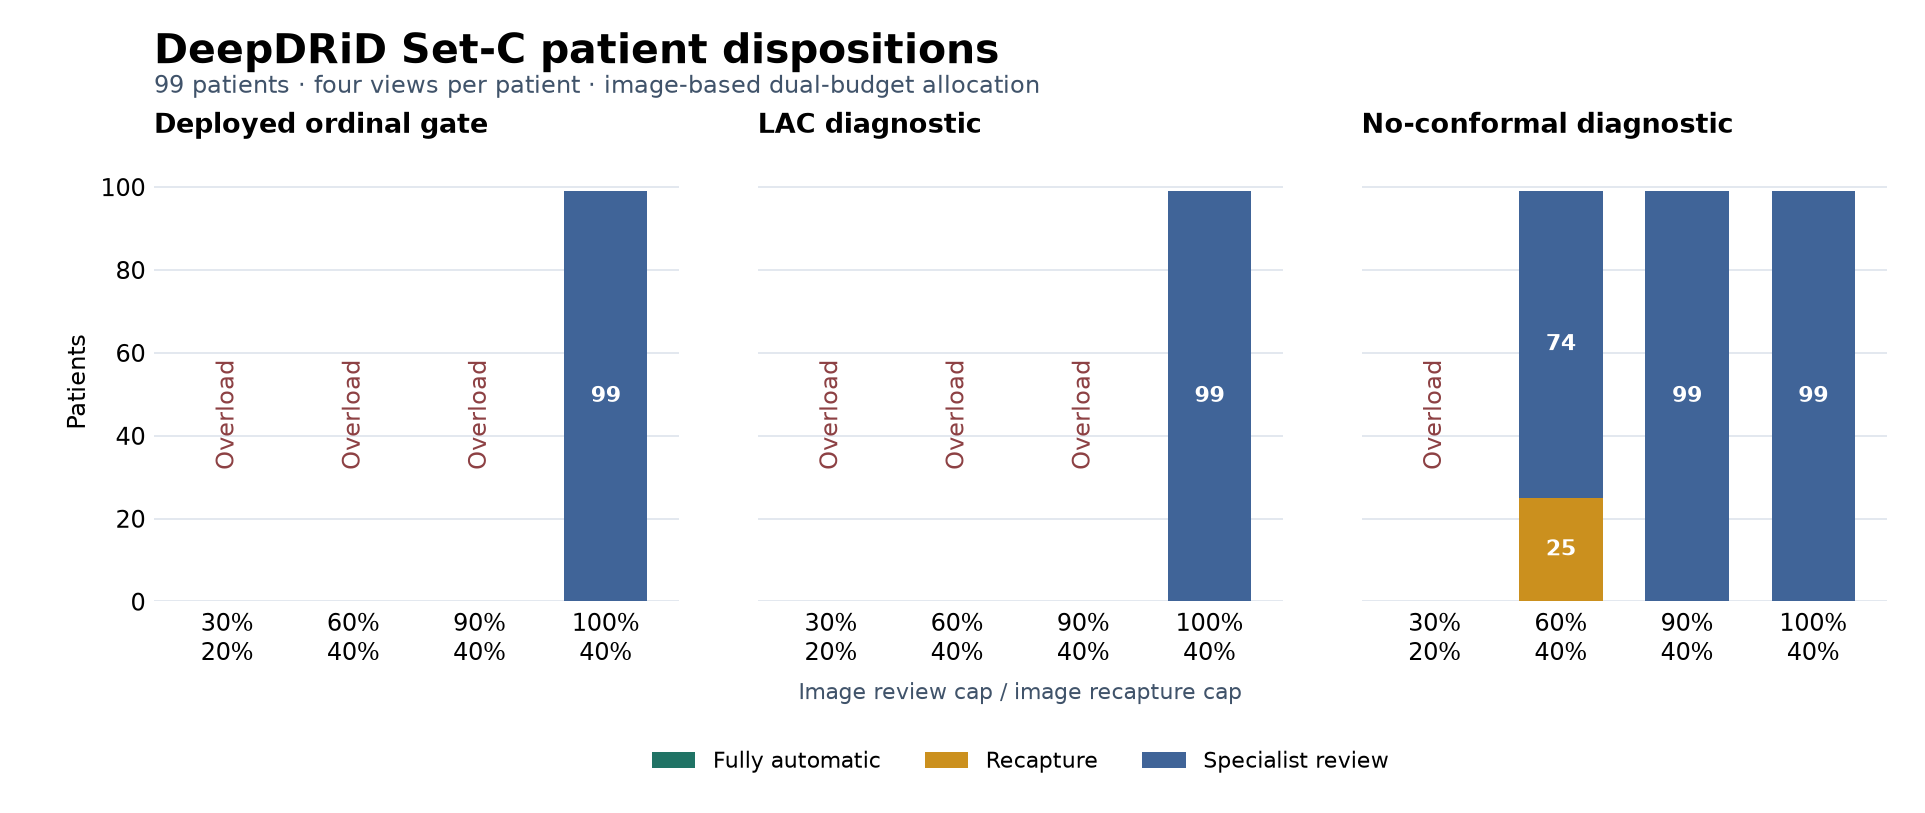
\includegraphics[width=\textwidth]{reports/set_c_validation_v1/patient_dispositions.png}
\caption{Patient recommendations under the deployed ordinal gate and two diagnostic variants.}
\label{fig:qsart-set-c}
\end{figure*}

\begin{figure*}[t]
\centering
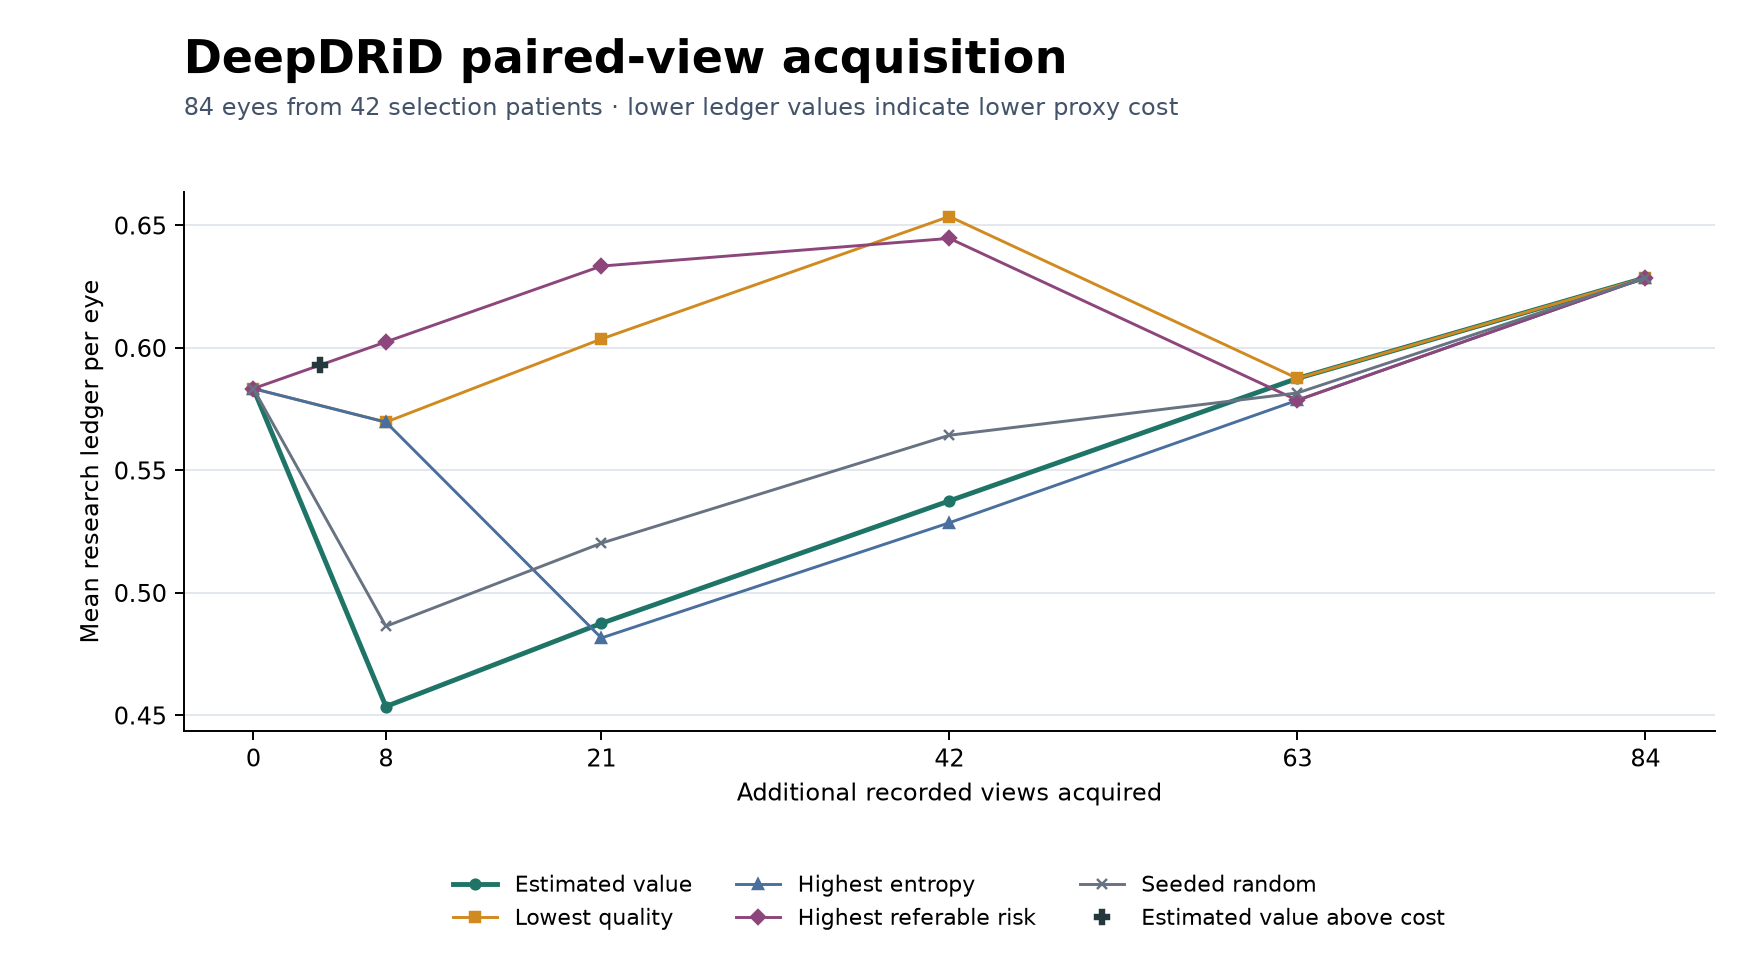
\includegraphics[width=\textwidth]{reports/paired_view_v1/acquisition_workload.png}
\caption{Research ledger by the number of additional recorded views.}
\label{fig:qsart-paired-views}
\end{figure*}


\subsection{Classification, Calibration, and Workload on Set-C}
Five-grade accuracy was 242/396 (61.1\%), with macro-F1 of 0.511 and quadratic
weighted kappa of 0.715. Worst-predicted-view
patient agreement was 52/99 (52.5\%). The grade-based patient referability
endpoint detected 45/48 referable patients and flagged 15/51 non-referable
patients. Maximum within-patient photo referable probability yielded an AUROC
of 0.956. Fixed-threshold image-quality accuracy was 299/396 (75.5\%).
Production temperature scaling reduced photo log loss from 1.067 to 1.022.

Ordinal prediction sets contained all five grades on every photograph,
yielding all-view inclusion in 99/99 patients. LAC achieved all-view inclusion
in 89/99 patients, with a mean set size of 3.43 and inclusion in 16/20 grade-4
photographs. Both dual-budget gates overloaded at the three lower image review
caps. At full review capacity both assigned all 99 patients to specialist
review, so the conditional clearance miss rate was undefined.
In Table~\ref{tab:qsart-set-c}, caps refer to review and recapture capacity
among photographs, while the allocation columns count patients. The rollups
for the ordinal and diagnostic gates appear in Fig.~\ref{fig:qsart-set-c}.

Without conformal sets, the 60\% review and 40\% recapture image caps admitted
45 automatic, 114 recapture, and 237 review recommendations. Four referable
photographs, including one severe photograph, received the automatic action.
Patient rollup yielded 74 review and 25 recapture recommendations with zero
fully automatic patients. This fit both image caps and exceeded the
corresponding 59-patient review capacity.

Across study modes, budgets, and methods, 39/96 scenarios were feasible
and 57 overloaded. At most one patient received full automatic clearance
in any feasible scenario. Of the 84 comparisons, 50 had overload in at
least one arm, 22 had unequal realized workloads, and 12 matched both
workloads at both units. The 12 matches gave identical image recommendations
and zero observed paired differences.

\subsection{Same-Eye Acquisition on Development Patients}
On 84 selection eyes, first-view prediction missed eight referable eyes,
including four severe eyes. With eight extra recorded fields, the value
ranking missed six referable eyes, including three severe eyes. The review
proxy rose from 36 to 38, and mean ledger cost decreased from 0.5833 to
0.4536 per eye. Each condition missed one patient in the severe subgroup.
Table~\ref{tab:qsart-paired-views} reports additional field counts, all
referable eye misses, severe eye misses within that group, and mean proxy
ledger cost per eye. Figure~\ref{fig:qsart-paired-views} shows the workload
curve.

At the same eight-field workload, the cost difference for value minus entropy
was $-0.1161$ per eye, with a paired 95\% interval of $[-0.3530,+0.0095]$.
At 21, 42, and 63 additional fields, entropy had the lower observed ledger
cost. All 16 matched cost intervals included zero. The positive-value cutoff
selected four fields, retained eight missed referable eyes, and increased
mean ledger cost to 0.5929 relative to first-field prediction.

\subsection{Context From Separate Studies}
Earlier DeepDRiD development studies measured additional model forwards
using horizontal flips of existing photographs and robustness under
controlled degradation. Severe JPEG compression reduced five-grade accuracy
from 63.10\% to 22.02\% in the degradation study. The paired-view study
counts additional recorded fields.

On FDR26 v3~\cite{FDR26v3}, a separate analysis measured 794/2,849 (27.87\%)
agreement between the frozen DeepDRiD classifier and released ALFEDIAM codes.
The prespecified APTOS-trained EfficientNet-B0 state evaluated on
IDRiD~\cite{R04} reached 42.97\% accuracy on 505 fingerprint representatives.
These results come from previously inspected cohorts, source-specific grades, and different
populations. Patient linkage was unavailable for the relevant analyses.

\section{Discussion and Limitations}
The ordinal gate included every supplied grade by returning every label.
This coincided with infeasible allocations at lower review capacity and
zero automatic patient dispositions at full capacity. The no-conformal
diagnostic cleared some referable photographs and required more review
slots when rolled up to patients than the corresponding patient budget
allowed. In multi-view cohorts, capacity reported for individual photographs
can differ from the capacity needed for patients.

The value ranking improved the eight-field proxy ledger relative to
first-field prediction. Matched comparisons against competing rankings
leave comparative benefit uncertain. The acquire-above-cost rule added
work without reducing measured misses. Classifier and value-estimator
fitting used the same training patients, and acquisition evaluation reused
classifier selection patients. The same-release Set-C split, residual risk
of undetected overlap, small severe strata, and correlation among views
limit interpretation.

Released grades were the observed outcomes. Completed recaptures, actual
clinician decisions, follow-up, and prospective acquisition remained
unobserved. The ledger weights are research proxies. Filename suffix order
defines the recorded-field replay, and true capture chronology remains
unknown. Prospective patient evidence is needed to estimate workflow effects.

\section{Reproducibility and Declarations}
Before scoring, the Set-C and acquisition methods were locked in the
\href{https://github.com/Riteshhai/Retina-Opthalmology/commit/eafd13db260bde7ed3627252d027e0cfc2ad2582}{Set-C source commit}
and the
\href{https://github.com/Riteshhai/Retina-Opthalmology/commit/6017d0c889d539b9d8c74ab33907015388040acf}{paired-view source commit}.
The \evidencelink{reports/set_c_validation_v1/evaluation.json}{Set-C report} and
\evidencelink{reports/paired_view_v1/evaluation.json}{paired-view report}
bind source, input, model, and runtime metadata. Independent auditors
reconstructed decisions and metrics from local witnesses and recorded the
aggregate SHA-256 digests in the
\evidencelink{reports/set_c_validation_v1/independent_audit.json}{Set-C receipt}
and
\evidencelink{reports/paired_view_v1/independent_audit.json}{paired-view receipt}.
The \evidencelink{docs/research/QSART_X_EVIDENCE_TABLE.md}{evidence table}
identifies the source fields. Original images, per-patient rows, and private
witnesses remain local. The
\evidencelink{docs/QSART_X_DATASETS.md}{dataset guide} describes access terms.

The authors must confirm authorship, affiliations, correspondence,
contributions, funding, conflicts of interest, and any applicable
institutional ethics, consent, or exemption statements before submission.

\IEEEtriggeratref{3}
\bibliographystyle{IEEEtran}
\bibliography{docs/research/references}
\end{document}
